%!TEX root = EmbSW1
\section{Scheduling}

\subsection{Multitasking}
\begin{itemize}
  \item Grundproblem:
  \begin{itemize}
    \item Wie werden die gemeinsamen Ressourcen am besten zugeteilt?
    \item Für die Zuteilung können unterschiedliche Strategien verwendet werden.
    \item Der \textbf{Scheduler} nimmt diese Zuteilung vor
    \item In den folgenden Betrachtungen gehen wir von der Zuteilung der Ressource \textbf{CPU} aus
  \end{itemize}
\end{itemize}

\subsubsection{Leistungsmerkmale}
\begin{itemize}
  \item Durchsatz (throughput): Anzahl erledigte Tasks pro Zeiteinheit
  \item Auslastung (utilization): Prozentuale Auslastung einer Ressource
  \item Mittlere Wartezeit (average waiting time)
  \item weitere
\end{itemize}

\subsection{Zweck von Real-time Scheduling}
\begin{itemize}
  \item Alle kritischen Zeiteinschränkungen (deadlines, response time) sollen eingehalten werden
  \item Im Notfall muss der Scheduling-Algorithmus entscheiden, um die kritischsten Tasks einhalten zu können
  \item Unter Umständen müssen dabei Deadlines von weniger kritischen Tasks verletzt werden
\end{itemize}

\subsection{Schedulability}
\begin{itemize}
  \item Eine Menge von Tasks ist dann schedulable, wenn alle Tasks zu allen Zeiten ihre Deadlines einhalten können
  \item Deadline:
  \begin{itemize}
    \item spätest mölicher Abschlusszeitpunkt
    \item bei periodischen Tasks ist das meist gleichzeitig mit dem Beginn der nächsten Periode
  \end{itemize}
\end{itemize}

\subsection{Scheduling-Strategien}
Die Zuteilung kann mit einem beliebigen Algorithmus erfolgen
\begin{itemize}
  \item FCFS (First Come First Served)
  \begin{itemize}
    \item einfachste Variante
  \end{itemize}
  \item Round Robin
  \begin{itemize}
    \item Rund herum in fixer Reihenfolge
  \end{itemize}
  \item SJF (Shortest Job First)
  \begin{itemize}
    \item wenn die kürzesten Tasks zuerst bearbeitet werden, wird die mittlere Wartezeit minimiert
  \end{itemize}
  \item Priority Scheduling
  \begin{itemize}
    \item unterbrechbar (preemptive) oder nicht unterbrechbar (non preemptive)
    \item tief priorisierte Tasks können verhungern
  \end{itemize}
  \item Random, u.a.
\end{itemize}

\subsection{Cooperative Multitasking}
\begin{itemize}
  \item In abgeschlossenen Systemen kann die Zuteilung durchaus kooperativ erfolgen
  \item Aktiver Task entscheidet selbst, wann er den Prozessor für andere Tasks frei gibt.
  \item Ein unfairer Task blockiert dabei die anderen (auch ein abgestürzter, aktiver Task)
  \item Nächsten Task aussuchen via: FCFS, Round Robin, zufällig, Prioritäten, etc.
  \item Sehr einfach zu implementieren
\end{itemize}

\subsection{Preemptive Scheduling}
\begin{itemize}
  \item Viele RTOS wenden präemptives Multitasking an (to preempt = zuvorkommen)
  \item Task mit höherer Priorität wird immer ausgeführt Task mit niedrigerer Priorität wird verdrängt (preempt)
  \item Prioritätsverteilungsmöglichkeiten
  \begin{itemize}
    \item Dynamic-priority algorithm: Prioritäten werden zur Laufzeit z.B. aufgrund vorhandener Deadlines angepasst.
    \item Static-priority algorithm: Prioritäten werden zur Entwicklungszeit estgelegt und nicht mehr geändert. $\rightarrow$ Einfacher als dynamic-priority
  \end{itemize}
  \item Viele RTOS verwenden static-priority Algorithmen, wir betrachten im folgenden nur noch diese
\end{itemize}

\subsection{Rate-monotonic scheduling}
\begin{minipage}{0.8\linewidth}
\textbf{Theorem:}
Hat man ein Set periodischer Task und static-priority preemptive scheduling, erhält man optimales Scheduling, wenn man die Prioritäten so verteilt, dass die Tasks mit kürzester Periodizität die höchste Prioriät erhalten (rate monotonic).\\
\textbf{RMA bound:}
Ein Set von n periodischen Tasks ist ohne weitere Abklärungen immer RM schedulable, wenn die Gesamtauslastung U folgenden Wert nicht überschreitet:
\begin{equation}
U(n) = n\cdot (2^{\frac{1}{n}}-1)
\end{equation}\\
Wenn U darüber liegt, muss mittels Analyse ermittelt werden, ob ein Schedule vorliegt.\\

Die maximale Systemauslastung beträgt:
\begin{equation}
\lim_{n \to \infty}n\cdot(2^\frac{1}{n}-1) = \ln 2 \approx 0.69
\end{equation}
Folgerung aus diesem Grenzwert: Wenn die Auslasting unterhalb von 69.3\% liegt, ist die Konfiguration auch bei unendlich vielen Tasks RM schedulable.
\end{minipage}
\begin{minipage}{0.2\linewidth}
\centering
\begin{tabular}{| c | c |}
\hline
n & U(n) [\%]\\
\hline
2 & 82.4\\
3 & 78.0\\
4 & 75.7\\
5 & 74.4\\
10 & 71.7\\
$\infty$ & 69.3\%\\
\hline
\end{tabular}
\end{minipage}

\subsubsection{Beispiel RMS}
\begin{itemize}
  \item T$_1$ hat die kleinste Periode und hat deshalb die höchste Priorität, dann kommt T$_3$, dann T$_2$
  \item Als erstes soll deshalb T$_1$, dann T$_3$, dann T$_2$ aufgezeichnet werden
  \item Ab dem Zeitpunkt 20 wiederholt sich das ganze Muster wieder
  \item Man beachte, dass zum Zeitpunkt 4 der am niedrigsten priorisierte Task T$_2$ unterbrochen wird (T$_1$ preempts)
  \item Die Gesamtauslastung des Systems ist 90\%, wobei alle Deadlines eingehalten werden
\end{itemize}
\begin{minipage}[t]{0.3\linewidth}
	\begin{tabular}{| l | l | l | l |}
		\hline
		Task & $e_i$ & $p_i$ & $u_i=\frac{e_i}{p_i}$ \\
		\hline
		T$_1$ & 1 & 4 & 0.25 \\
		\hline
		T$_2$ & 5 & 20 & 0.25 \\
		\hline
		T$_3$ & 2 & 5 & 0.40 \\
		\hline
	\end{tabular}
\end{minipage}
\begin{minipage}[c]{0.7\linewidth}
	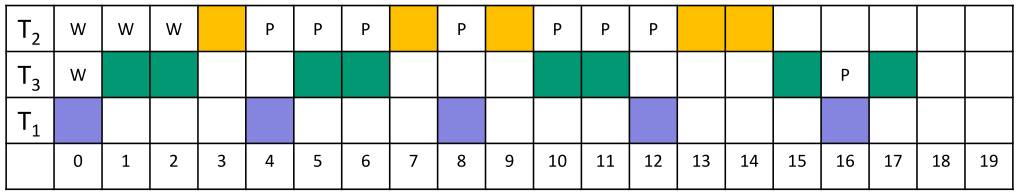
\includegraphics[width=\linewidth]{images/Schedule/RMS}
\end{minipage}

\subsubsection{Anleitung für die Zuweisung von Prioritäten bei RM Scheduling}
\begin{enumerate}
  \item Prioritäten immer gemäss RMS zuweisen. Manuelle Zuweisung gibt keine bessere Lösung!
  \item Falls die Auslastung nicht grösser ist als die RMA Grenze, dann ist alles perfekt, die Konfiguration ist RM schedulable
  \item Falls die Auslastung grösser ist, muss manuell analysiert werden, ob die Konfiguration schedulable ist
  \item 100\% Auslastung könnte erreicht werden, wenn alle Perioden harmonisch sind, d.h. jede längere Periode ist ein exaktes Vielfaches aller Perioden kürzerer Dauer, z.B. (10, 20, 40, 80)
  \item Harmonische Perioden verringern die Unterbrechung (Preemption) von niedrig priorisierten Tasks\\
  Beispiel: (10, 20, 40) ist gegenüber (10, 20, 50) zu bevorzugen, wenn das möglich ist
\end{enumerate}


\subsubsection{Interrupts}
Da die ISR von der Hardware getrieben wird, ist auch der niederwertigst priorisierte Interrupt
immer noch höher priorisiert als der höchst priorisierte Task. Für die RM-Analyse stehen 2 Lösungsvarianten zur Verfügung:
\begin{itemize}
  \item[1.]  Der ISR-Code wird nicht mittels Interrupt ausgelöst, sondern in einem Polling-Loop.
  \item[2.]  Für die RM-Analyse wird mit der Periode der höchsten Priorität gerechnet.
\end{itemize}
